% Auth: Nicklas Vraa
% Docs: https://github.com/NicklasVraa/LiX

\documentclass{textbook}

\lang      {english}
\title     {Modeling, Simulation and Optimization}
\subtitle  {(For the Layman)}
\author    {Jaime Torres}
\cover*    {resources/textbook_front.pdf}{resources/textbook_back.pdf}
\license   {CC}{by-nc-sa}{3.0}{The Company}
\isbn      {978-0201529838}
\publisher {Nobodym just me!}
\edition   {1}{2024}
\dedicate  {Myself}{Because I'm cool}
\thank     {Thank you to me for being the best}
\keywords  {optimization, simulation, python, mathematical modeling}

\begin{document}

\tableofcontents

\part{Mathematical Models}

\chapter{Introduction to Mathematical Modeling.}

For this chapter, we'll:

\begin{itemize}
    \item Get our framework from an algorithmic framework of thinking to algebraic 
    framework
    \item Represent a problem with algebraic expressions.
    \item Make proper implementations of mathematical models.
\end{itemize}

\section{Definitions to mathematical modeling}

Before we can begin to think about models, we must understand what they are.
And, for the purposes of this book, we can define a mathematical model as a representation
of a real life problem with an abstract representation of the phenomenons we intend to study.

For an immediately relevant example, a lot of problems in graph theory can be explained in algebraic terms.
Although these problems can be a bit more mathematical in nature, then we can use them to explain real-life problems.
Such as:

\begin{itemize}
    \item Shortest path in a graph, for computer networking and pathfinding.
    \item The traveling salesman problem, for pathfinding, DNA sequencing and microchip manufacturing 
    \item The vehicular routing problem, for finding multiple instances of a TSP-esque solution on a same graph
\end{itemize}

As a practical example of such a graph-based problem, let's analyze the following:

\subsection{Example 1: The transport problem}

Let a finite number of sources and a finite number of destinations, we can determine the
number of elements we can route to every destination with a minimal cost for every source. 
For example, if we said such sources are factories and the destinations are warehouses, we could see a 3x3
graph as it follows:

% \includegraphics[options]{name}

\subsection{Example 2: Cover problems}

More than a specific problem, this is a subdivisio of problems meant to cover a certain group of demands
or coverage criteria according to a specific defined problem.

\subsubsection{The hospital problem}

For example, say we got a group of neighborhoods that are of euclidian behavior, and we intend to put the minimum amount of
hospitals that can cover the entire region we're considering. A hospital covers the neighborhood is located on and
those who share a boundary with it. A boundary is a non-zero

For an example, imagine the following instance of this problem:

%% answer is 5 and 8

\subsubsection{The four color theorem}

The four color theorem is a very famous application of a cover problem. 

% 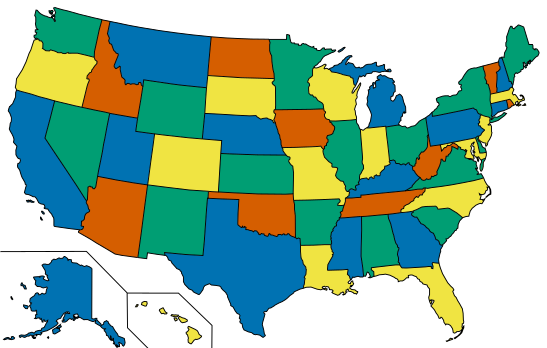
\includegraphics[scale=0.4]{notes/resources/Map_of_United_States_accessible_colors_shown}

\subsection{Example 3: Minimum spanning tree}

If we imagine a tree data structure such as a graph with no cycles, and a graph as an interlocked set of
nodes, a minimum spanning tree would be the minimum cost path that can connect all nodes as a tree.

This problem has a set of requirements for it to be considered correct:

\begin{itemize}
    \item There must be no cycles or subcycles in the solution
    \item the number of connections must be the number of nodes minus one
\end{itemize}

\section{Classification of mathematical models}

These models can be, as most things in mathematics, categorized and calificated in 

\subsection{Deterministic mathematical models}

These are models that can be predicted in a way that is certain.

\subsection{Stochastic mathematicam models}

A stochastic model is one that involves a certain amount of randomness. For example, 

\subsection{Static mathematical models}

A static model is one that does not depend on time, implying that whatever time passes, the result of
such a system should stay constant. Generally this will happen for models where we don't even consider time as a 
relevant variable.

\subsection{Dynamic mathematical models}
\subsubsection{Continuous time models}

A continuous time model is one where we assume time as a continuous function, that meaning, it is
flowing in somewhat real time. Although the way computation has it should bring it to be a finite level of
statuses, this should be a big enough sample such as we can assume the variable can be statistically generalized into
a continuous system

\subsubsection{Discrete time models}

A fairly interesting application of discrete time models comes from finance, where there exists 
capitalization in a set time interval. For example, we could imagine the free cash flow of an economic project as
a mathematical problem to be optimized, such as this:

\subsubsection{Continuous status models}

In a continuous status model, the dependant variable can assume any value in the range of a specific interval.

\subsubsection{Discrete status models}

In these models, the difference is analogous to the way a discrete time model varies from a continuous
time model. Values for the dependant variable shouls only assume specific values in an interval. For example, a
model where every value the dependant variable can take is in the range of natural numbers ($\mathbb{N}$) would be 
a discrete status.

\subsubsection{Examples of model classification}

\paragraph{Number of attendants in a bank every hour}

This example would be a dynamic mathematical model where every 

\paragraph{Temperature of a classroom every hour}

For this, 

\subsection{Open mathematical models}

An open mathematical model is one where the input that is recieved will be external to this model and
independent from itself. For example a translator, such as Google Translate or DeepL will model natural language
such as the input recieved is not eventually retroactively giving feedback to the model. Although it is possible that
in ML models there are eventually expected use cases introduced into the model, for out purposes, they will be considered 
open as long as at runtime the previous example does not feedback into further answers.

\subsection{Linear mathematical models}

Assume the following definition of linearity

A function 'f(x)' is linear if:
\begin{itemize}
    \item Ex. 1: $f(u+v) = f(u) + f(v)$
    \item Ex. 2: $f(k \cdot u) = k \cdot f(u) ; k \ is \ constant$
    \item $\not \exists \ x \in \mathbb{R}  \implies (Ex. 1 \ f(x+y); x,y \in \mathbb{R} \neq f(x) +f(y)) \lor (Ex. 2 \ f(k \cdot x); k, x \in \mathbb{R} \neq k \cdot f(x)) $
\end{itemize}

a linear mathematical model should have every single function following these constraints. 

%\includegraphics[options]{name}

\chapter{Optimization Solutions in Mathematical Models}

Now, given that we know what a problem in modeling entails, how can we begin
to solve it? As it might be evident by now, this question will be the crux of most our
problems, and yet there is not much to fear. As it comes, we really have tought about quite an
important amount of problems already, and they provide a baseline for our analysis. As with
many problems in computer science, we stand in the shoulders of giants, really.

So for example, we can imagine the following case:

\section{Parts of an Optimization problem}

\textbf{\textit{Example 1:}}
Let the following problem:

\textit{"We have 8 projects that return a certain profit, so we want to select as many projects as possible that will return a certain profit.
we want to select as many projects as possible that will generate the highest profit.
generate the highest profit. Suppose that the profit of each project is
and we have a constraint for acquiring the projects, which is that we can only choose 2 projects.
that we can only choose 2 projects.
Propose a mathematical optimization model to solve the problem."}

\textbf{Note:} We assume equal spending for them.

\begin{gather}
    F_{j}(x); \forall j \in \mathbb{N}
\end{gather}

The first thing to do is to determine the different parts of this program, for those purposes, we can
determine them in the following categories:

\begin{itemize}
    \item Sets: the group of sets that can be applied to this problem, assuming sets as a group of mathematical variables.
    \item Indexes: the identifier for which we call every item inside of a set
    \item Parameters: the numerical and mathematical significance of every index inside of a set.
    \item Decision Variable: the variable we mean to analyze in our problem.
    \item Objective function: The expected behavior of a decision variable
    \item Restrictions: The rules under which we analyze the previous ideas.
\end{itemize}

as such, for this problem we can imagine the categories proposed previously as such:

\begin{itemize}
    \item Sets: P is a set of projects, that can be represented as $$P = {1,2 \dots 8}$$
    \item Indexes: i is a number from 1 to 8 that represents the order of the project to be selected
    \item Parameters: $g_i$ will be our representation of profit under this system.
    \item Decision Variable: $x_i$ will be a binary (either 1 or 0) constant that will represent the selection of a project.
    \item Objective function: $$max(\sum_{i \in P} g_{i} \cdot x_{i})$$ This means we intend to optimize 'g', which represents profit, and is bound to an 'x' binary constant.
    \item Restrictions: $$\sum_{i \in P} x_i = 2$$ This means that we can only choose two projects, it makes sense because those values will multiply $g_i$ in our objective function
\end{itemize}

Now, say we want to represent this model in Pyomo, a python library for this sort of optimization. Say


\code{my_code}{python}{

    from __future__ import division
    from pyomo.environ import *

    from pyomo.opt import SolverFactory

    Model = ConcreteModel()

    # Data de entrada
    numProjects=8

    p=RangeSet(1, numProjects)

    value={1:2, 2:5, 3:4, 4:2, 5:6, 6:3, 7:1, 8:4}

    # Decision Variable
    Model.x = Var(p, domain=Binary)

    # Objective Functions
    Model.obj = Objective(expr = sum(Model.x[i]*value[i] for i in p), sense=maximize)

    # Restrictions
    Model.res1 = Constraint(expr = sum(Model.x[i] for i in p) == 2)

    # Solver specifications
    SolverFactory('glpk').solve(Model)

    Model.display()
    }
    {Representation of the proposed solution in code.}

a script for this program can be found in the repository for this book. The resulting output will be as follows:

\code{my_code}{plaintext}{
    Model unknown
    Variables:
        x : Size=8, Index=[1:8]
            Key : Lower : Value : Upper : Fixed : Stale : Domain
            1   :     0 :   0.0 :     1 : False : False : Binary
            2   :     0 :   1.0 :     1 : False : False : Binary
            3   :     0 :   0.0 :     1 : False : False : Binary
            4   :     0 :   0.0 :     1 : False : False : Binary
            5   :     0 :   1.0 :     1 : False : False : Binary
            6   :     0 :   0.0 :     1 : False : False : Binary
            7   :     0 :   0.0 :     1 : False : False : Binary
            8   :     0 :   0.0 :     1 : False : False : Binary
    
    Objectives:
            obj  : Size=1, Index=None, Active=True
            Key  : Active : Value
            None :   True :  11.0
    
    Constraints:
            res1 : Size=1
            Key  : Lower : Body : Upper
            None :   2.0 :  2.0 :   2.0
}{Output of the provided problem}

this implies that for the example program, we will choose projects 2 and 5. 

\section{Mathematical management of expressions.}

Now as it might be evident, the fact is we'll be using mathematical expressions 
in order to make sense of our problems. This means we need to understand
how 

Generally, 

\begin{itemize}
    \item Sumatory: $\sum_{i\in \mathbb{N}} x_i = j ; j \in \mathbb{R}$
    \item For every item: $x_i = j ; \forall_{i \in \mathbb{N}}$
\end{itemize}

\subsection{Conditional Operations}

The before noted expressions are general, that means, when ran over a subset of data, they will
take all items and apply an operation over them. however, we won't always want this sort of behaviour in our
systems.

\begin{itemize}
    \item Conditional Sumatory: $\sum{i \in \mathbb{N}} x_i ; \forall i \in \mathbb{N} | i = x$
    \item Conditional for every item: $\forall{x_i = j; i \in \mathbb{N} | i = y}$
\end{itemize}

\textbf{Example: }

Given the following cases:

\textit{given the set: $N = \{1 .. 10\}$ and the specific restriction 
$x_2 + x_3 + x_6 + x_8 + x_10 = 1$, how would we write the generic restriction?
}

We can use a conditional sumatory to represent this restriction, such as it follows:

\begin{gather}
    \sum_{i \in N} x_i = 1 ; \forall i \in N | i \in i \mod 2 = 0 | N = \{ 1 .. 10  \}
\end{gather}

\textit{Given the set $N = \{ 1,2,3 \}$, How would we expand the generic expression:}

$\sum_{i \in N}\sum_{j \in N}\sum_{k \in N} = x_{ijk} = 1$

This would be basically a matrix sum, written as such:

\begin{gather}
    x_{1,1,1} + x_{1,1,2} + x_{1,1,3} \\
    x_{1,2,1} + x_{1,2,2} + x_{1,2,3} \\
    \dots \\
    x_{3,3,1} + x_{3,3,2} + x_{3,3,3} = 1 \\
\end{gather}

The Amount of expressions is a combination from the different elements in N. In this case, it is a sum of
27 elements (3x3x3)

\textit{Given the set $N = \{ 1,2,3 \}$ and the specific restrictions:
$$ x_{12} + x_{13} = 1 \\  $$
} 

This is a 'for all' expression, such as:
\begin{gather}
    \sum_{i , j \in N} x_{i,j} = 1 | \forall_{i,j} \in N | j \neq 1
\end{gather}

\subsection{Usual errors when managing mathematical expressions.}

We can sometimes screw up, and that's okay when we're practicing. However,
it is also important to know why we could do so. 

\subsubsection{Not controlling an index}

On the examples here shown, we have implicitly expected an 'index' to be found somewhere. 
that is where 'i' and 'j' come from. 

\section{graph problems}

We will be working extensibly on graph problems on the duration of 
this 

\chapter{Examples}

\section[Homework 1]{Homework 1: The diet problem}

\subsection{Solution to the problem}
\code{my_code}{python}{
    from __future__ import division
    from pyomo.environ import *
    
    from pyomo.opt import SolverFactory
    
    '''
    # Definicion variables alimento
    
    c = carne = 1
    a = arroz = 2
    l = leche = 3
    p = pan = 4
    
    Todos los valores numericos vienen del enunciado.
    '''
    Model = ConcreteModel(name='dieta')
    
    '''
    N = Productos.
    
    1 = Carne
    2 = Arroz
    3 = Leche
    4 = Pan
    '''
    N = RangeSet(1,4)
    
    # Variable de decisión, ligada a N *****************************************************************************************************************************************
    
    Model.c = Var(N, domain=NonNegativeReals) 
    
    '''
    M = Caracteristicas de los productos.
    
    1 = Calorias
    2 = Proteinas
    3 = Azucar
    4 = Grasas 
    5 = Carbohidratos
    
    '''
    M = RangeSet(1,5)
    
    '''
    Precios, los valores de las llaves corresponden a aquellos en N 
    '''
    p =  {1:3000,2:1000,3:600,4:700} 
    
    '''
    Variable objetivo,
    '''
    Model.obj = Objective(expr = sum(Model.c[i]*p[i] for i in N), sense=minimize)
    
    
    '''
    Datos de las comidas, cada dato esta organizado de forma que pueda leerse en el orden 
    v[i][j]. donde 'i' es un valor de N (es decir, un alimento) y donde 'j' es un valor de M
    (es decir, una caracteristica)
    '''
    v = {
        1:{ 
            1:287,
            2:26,
            3:0,
            4:19.3,
            5:0
        },
        2:{
            1:204,
            2:4.2,
            3:0.01,
            4:0.5,
            5:44.1
        },
        3:{
            1:146,
            2:8,
            3:13,
            4:8,
            5:11
        },
        4:{
            1:245,
            2:6,
            3:25,
            4:0.8,
            5:55
        }
    }
    
    '''
    Limites.
    
    Ligados a M
    '''
    L = {
        1: 1500,
        2: 63,
        3: 25,
        4: 50,
        5: 200
    }
    
    def inferior(Model, j):
        if j != 1 and j != 2:
            return (sum(Model.c[i]*v[i][j] for i in N ) <= L[j]) 
        else:
            return Constraint.Skip    
    Model.inferior = Constraint(M, rule=inferior)
    
    def superior(Model, j):
        if j == 1 or j == 2:
            return (sum(Model.c[i]*v[i][j] for i in N) >= L[j])
        else:
            return Constraint.Skip
    Model.superior = Constraint(M, rule=superior)
    
    # Especificación del solver
    SolverFactory('glpk').solve(Model)
    
    Model.display()
}{Solution to the problem}

\end{document}
